\problemname{Bitaflipp}

Turing vél samanstendur af tveimur meginhlutum. Fyrst er band sem skipt hefur
verið í litlar einingar, og eru þær númeraðar í hækkandi röð frá $1$. Á hverri
einingu er skrifað annaðhvort tölustafurinn $0$ eða tölustafurinn $1$. Ofan á
þessu bandi er svo haus. Þessi haus er yfir einni einingu í einu, en hann getur
fært sig fram og til baka á milli eininganna. Hausinn getur einnig lesið af og
skrifað á eininguna sem hann er yfir. Þessa vél er svo hægt að forrita til að
leysa sömu verkefni og nútíma tölvur geta leyst.

\begin{figure}[h]
    \centering
    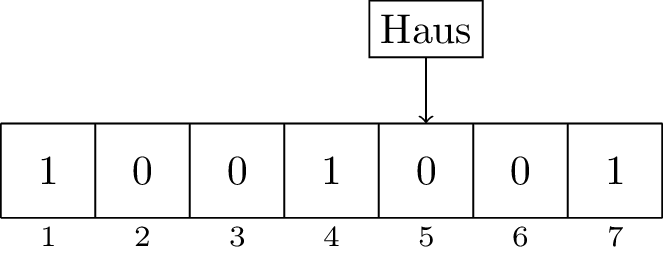
\includegraphics[scale=0.35]{machine.png}
    \caption{Mynd af Turing vél ásamt bandinu úr fyrsta sýnidæminu.}
\end{figure}

Gunnar litli er búinn að vera að æfa sig í að forrita svona Turing vél. Nýjasta
forritið hans byrjar með hausinn á einingu númer $i$. Hausinn skoðar töluna sem
skrifuð er í núverandi einingu. Ef hún er $1$, þá skrifar hausinn $0$ yfir
töluna, en ef hún er $0$, þá skrifar hausinn $1$ yfir töluna. Svo fer hausinn á
eininguna til hægri. Þetta er endurtekið alveg þar til hausinn er búinn með
einingu $j$.

Sem dæmi, segjum að Gunnar litli keyri forritið með $i=5$ og $j=7$ á bandinu sem
sýnt er í myndinn að ofan. Hausinn byrjar þá á einingu $5$. Hausinn breytir þar
$0$ í $1$, og fer á reit $6$. Þar breytir hausinn $0$ í $1$, og fer á reit $7$.
Þar breytir hausinn $1$ í $0$. Núna er hausinn búinn með reit $j=7$ og stoppar.
Á bandinu mun því standa \texttt{1~0~0~1~1~1~0} þegar vélin er búin.

Gunnar litli hefur mjög gaman af þessu. Hann er búinn að vera að keyra
forritið sitt með mismunandi böndum og mismunandi gildum á $i$ og $j$, sem
uppfylla þó $1 \leq i \leq j \leq N$ þar sem $N$ er fjöldi eininga í bandinu.
Núna er hann með band sem honum finnst mjög áhugavert, og hann veltir fyrir sér
hver er hæsti mögulegi fjöldi eininga sem innihalda töluna $1$ eftir að hann
keyrir forritið á þetta band, ef hann velur $i$ og $j$ á besta mögulegan hátt.

\section*{Inntak}
Í fyrstu línu er ein heiltala $N$ sem táknar fjölda eininga í bandinu. Þar
á eftir fylgir lína með $N$ tölum, sem eru annaðhvort $0$ eða $1$, sem táknar
upphaflega innihald eininganna í röð frá $1$ til $N$.

\section*{Úttak}
Úttak á að innihalda eina línu með heiltölu sem táknar hæsta mögulega fjölda
eininga sem innihalda töluna $1$ eftir að forritið er keyrt, ef $i$ og $j$ eru
valin á besta mögulegan hátt.

\section*{Útskýring á sýnidæmum}
Bandið í fyrsta sýnidæminu er sýnt í myndinni að ofan. Það inniheldur $7$
einingar. Í þessu sýnidæmi er hæsti fjöldi eininga með tölunni $1$ hægt að fá
með því að keyra forritið með $i=2$ og $j=6$, og eru þá $6$ einingar með töluna
$1$.

Í seinna sýnidæminu eru þegar allar einingarnar með töluna $1$. En Gunnar litli
þarf að keyra forritið nákvæmlega einu sinni. Ef hann keyrir forritið með $i=1$
og $j=1$ þá eru $2$ einingar eftir með töluna $1$, og er það hæsti fjöldinn
sem hægt er að enda með.

\section*{Stigagjöf}
Lausnin mun verða prófuð á miserfiðum inntaksgögnum, og er gögnunum skipt í
hópa eins og sýnt er í töflunni að neðan. Lausnin mun svo fá stig eftir því
hvaða hópar eru leystir.

\begin{tabular}{|l|l|l|}
\hline
Hópur & Stig & Inntaksstærð \\ \hline
1     & 25 & $ 1 \leq N \leq 100$ \\ \hline
2     & 25 & $ 1 \leq N \leq 1\,000$ \\ \hline
3     & 50 & $ 1 \leq N \leq 10^5$ \\ \hline
\end{tabular}

